\documentclass[a4paper]{article} % {scrartcl} % for \subtitle
\usepackage[italian]{babel} 
\usepackage[utf8]{inputenc}
\usepackage[T1]{fontenc}
\usepackage{graphicx}
\usepackage{subfigure}
\usepackage{amsmath,amssymb, amsthm}
\usepackage{tabularx}
% Customized hyper references
\usepackage[pdftex,colorlinks]{hyperref}
%% Collegamenti ipertestuali in blu
%% in modo che siano visibili anche stampati
\hypersetup{%
            citecolor=blue,%
            filecolor=blue,%
            linkcolor=blue,%
            urlcolor=blue}

\author{Gianmarco Brocchi}
\title{Weighted Nonnegative Matrix Factorization \\
and Face Feature Extraction \\ - \\ un'implementazione}
% \subtitle{Un'implementazione}
\date{\today}

\begin{document}
\maketitle

Usando l'algoritmo suggerito nell'articolo \ref{wnmf} si vuole applicare la WNMF ad una raccolta di immagini in modo da enfatizzare certe parti della matrice che le rappresenta. Useremo immagini di volti per evidenziare la parte centrale del viso.

\section{L'algoritmo}

\subsection{Kullback-Leibler Divergence}\label{KL-div}
Per studiare la convergenza del metodo vengono proposte regole di aggiornamento sotto le quali non aumentano, rispettivamente, la \emph{norma euclidea} e la \emph{Kullback-Leibler Divergence}; quest'ultima è una stima non simmetrica della differenza tra due distribuzioni di probabilità. Nello specifico, date due distribuzioni di probabilità $P$ e $Q$, la divergenza Kullback–Leibler di $Q$ da $P$, indicata con $D_{KL}(P \lVert Q)$, è una misura dell'informazione persa quando $Q$ è usata per approssimare $P$. Tale misura è scelta comune nell'approssimazione di immagini come nel nostro caso.

Data la matrice $A$, la sua distanza dalla fattorizzazione $UV$ è:
\[ D(A \lVert UV) := \sum_{ij} \left[ A \circ \log_{\circ} \frac{[A]}{[UV]} - A + UV \right]_{ij} \]

Per cui data $A$, stimeremo la sua distanza dalla fattorizzazione $UV$ con la \emph{KL-divergence} pesata con $W$ in questo modo:
\[ D_W(A \lVert UV) := \sum_{ij} \left[ W \circ \left( A \circ \log_{\circ} \frac{[A]}{[UV]} - A + UV \right) \right]_{ij} \]

Nota: con $\circ$ si indica di \emph{prodotto di Hadamard}, mentre con $\frac{[\;]}{[\;]}$ la \emph{divisione di Hadamard}, effetuatte componente a componente; con $\log_{\circ}$ si indica il logaritmo delle componenti.

\subsection{Update rules}\label{updaterules}
La divergenza pesata in \ref{KL-div} non aumenta con i seguenti aggiornamenti:

\[ \frac{[V]}{[U^tW]} \circ \left( U^t \frac{[W \circ A]}{[UV]} \right) \rightarrow V \text{ , } \frac{[U]}{[WV^t]} \circ \left( \frac{[W \circ A]}{[UV]}V^t \right) \rightarrow U \]

In \ref{wnmf} viene mostrato come la divergenza $D_W(A\lVert UV)$ non cresce con tali aggiornamenti se $U$ e $V$ sono non negative.

\subsection{Passi}
\paragraph{Conversione}\label{subsec:conversione}
Le immagini, per poter applicare l'algoritmo, sono state convertite da formato RAW in ASCII e rinumerate da $1$ a $400$ per un più semplice recupero delle stesse. Per la conversione delle immagini è stato usata la libreria \texttt{PGMA TO PGMB} (in \texttt{C++}).
[Vedi \ref{itm:A2B}].

Le immagini vengono lette e convertite in ``vector face'', salvati come vettori colonna nella matrice $A$; viene contemporaneamente creata la matrice dei \emph{locale} dei pesi $W$, i cui elementi sono dati da:

\[ localW(i,j) = e^{-\frac{d}{\sigma^2}} \]

dove $d$ è la distanza dal centro dell'immagine della componente $(i,j)$ e $\sigma$ viene fissato a $30$.
Anche questa matrice viene convertita e salvata come ``vettore peso'' nella matrice $W$.

\paragraph{Iterazioni}
Fissato un numero massimo di passi e la precisione massima si applicano le regole in \ref{updaterules}.\\
Vengono stampati a video la KL-divergence e il massimo della matrice $UV$ ad ogni passo.

\paragraph{Stampa}
Raggiunta la precisione richiesta o superato il numero di iterazioni la fattorizzazione ottenuta viene stampata su file.
Per il confronto viene eseguita un'ulteriore fattorizzazione con matrice dei pesi fissata a $\textbf{1}$ (senza pesi).

\paragraph{Librerie}
Per leggere e scrivere i file PGM è stata utilizzata la libreria \texttt{PGMA IO} (per Fortran90).
[Vedi \ref{itm:IO}].

\section{I dati}
L'algoritmo lavora su dati ottenuti dall'\texttt{ORL} face database\footnote{un insieme di volti dall'Olivetti Research Laboratory di Cambridge, UK}. [Vedi \ref{ORL}].
Nello specifico si tratta di $400$ volti ($10$ immagini di $40$ soggetti). Le immagini sono in formato PGM\footnote{Portable Gray Map format}, ovvero in scala di grigi; tali immagini possono essere in formato RAW o ASCII, nel primo i valori di grigio sono memorizzati come semplici byte, nel secondo sono rappresentati da numeri tra 0 e 255. \\ 
(Nota: le immagini dell'\texttt{ORL} erano nel primo formato, pertanto è stato necessario convertirle: vedi \ref{subsec:conversione})

\section{Test}

Per testare il progetto è possibile clonare il necessario via \texttt{git} all'indirizzo:
\begin{center} \url{http://poisson.phc.unipi.it/~brocchi/git/WNMF/} \end{center}

\paragraph{Makefile}
Dalla cartella è possibile dare i seguenti comandi:
\begin{description}
\item[\texttt{make}]: compilerà i sorgenti \texttt{Fortran90} e li linkerà nell'eseguibile \texttt{PGM}
\item[\texttt{make run}]: esegue un \texttt{make} e lancia in automatico l'eseguibile
\item[\texttt{make faces}]: si occupa di scaricare il database dei volti, scompattarlo, compilare il convertitore e convertire le immagini in \texttt{ASCII}, rinumerandole in ordine crescente nella cartella \texttt{faces}
\item[\texttt{make clean}]: elimina e pulisce file binari e temporanei
\item[\texttt{make whole}]: esegue sia un \texttt{make faces} che un \texttt{make}, aggiungendo \texttt{run} esegue direttamente il programma.
\end{description}


% Al fine di ottenere la miglior velocità di convergenza (e quindi il minor valore della \emph{KL-divergence} dopo un numero fissato di passi) sono state testate diverse implementazioni dell'algoritmo. In particolare, come accennato in \ref{libnmf}, le matrici $U$ e $V$ possono essere:
% \begin{itemize}
% \item generate entrambe in maniera random
% \item generata random una e calcolata l'altra
% \end{itemize}
% Sono stati provati enbrambi gli approci.\\
% Si è anche provato a ricalcolare $V$ a intervalli regolari durante gli aggiornamenti per migliorare la convergenza.
% Inoltre sono state testate le varianti aggiornando $U$ e $V$ separatamente (ovvero senza usare l'ultimo aggiornamento di $U$ per aggiornare $V$) e scambiando l'ordine di aggiornamento.
Fissato un numero di iterazioni vengono confrontate le divergenze ottenute usando o meno la matrice dei pesi $W$:

\begin{center}
  Risultati con $10$ immagini e rango $9$: \\

  \begin{tabular}{| l | c | r |}
    \hline
    Iterazioni & $D_W(A\lVert UV)$ & $D(A\lVert UV)$ \\
    \hline
    61 & 17810.75 & 68617.87 \\
    81 &  9578.67 & 40448.83 \\
    201 & 4619.00 & 23890.91 \\
    \hline
  \end{tabular}
  \vspace{0.5cm}

  Risultati con $100$ immagini e rango $49$: \\

  \begin{tabular}{| l | c | r |}
    \hline
    Iterazioni & $D_W(A\lVert UV)$ & $D(A\lVert UV)$ \\
    \hline
    20 & 1000594.20 & 3927411.60 \\
    50 &  523867.72 & 1965531.56 \\
    \hline
  \end{tabular}

\end{center}

% \newpage
\section{Conclusioni}
Abbiamo visto come, usando la WNMF, sia possibile enfatizzare certe caratteristiche in un'immagine, migliorandone l'accuratezza nei problemi di approssimazione.

\subsection{Esempi}
Alcuni esempi di immagini:

\begin{figure}[h]
  \centering
  \subfigure[Senza pesi]
  {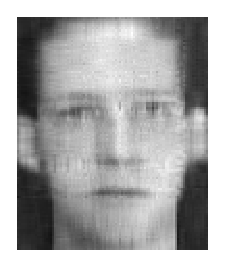
\includegraphics[scale=1.10]{img/singUV_noW_80.eps}}
  \subfigure[Con pesi centrati]
  {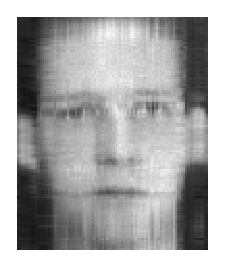
\includegraphics[scale=1.10]{img/singUV_80.eps}}
  \hspace{2mm}
  \subfigure[Originale]
  {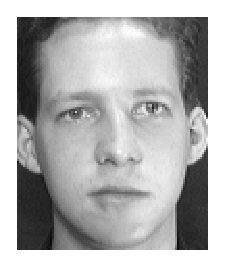
\includegraphics[scale=1.10]{img/original.eps}}
  \caption{Immagini dopo 80 iterazioni a confronto}
\end{figure}

\begin{figure}[h]
  \centering
  \subfigure[Senza pesi]
  {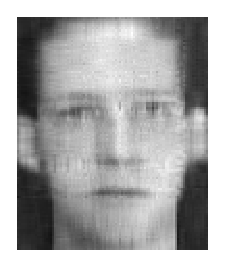
\includegraphics[trim = 5mm 20mm 5mm 12mm, clip=true, scale=1.60]{img/singUV_noW_80.eps}}
  \subfigure[Pesi centrati]
  {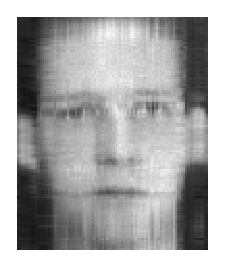
\includegraphics[trim = 5mm 20mm 5mm 12mm, clip=true, scale=1.60]{img/singUV_80.eps}}
  \subfigure[Originale]
  {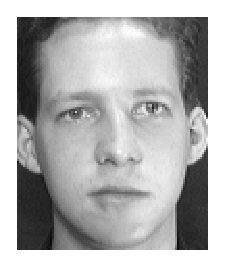
\includegraphics[trim = 5mm 20mm 5mm 12mm, clip=true, scale=1.60]{img/original.eps}}
  \caption{80 iterazioni, occhi a confronto}
\end{figure}

% \begin{figure}
%   \centering
%   \subfigure[Senza pesi]
%   {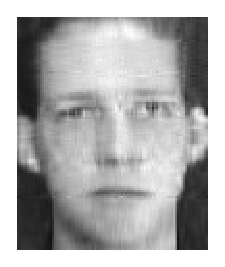
\includegraphics[scale=1.00]{img/singUV_noW_200.eps}}
%   \subfigure[Con pesi centrati]
%   {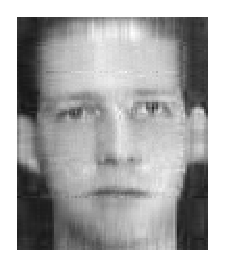
\includegraphics[scale=1.00]{img/singUV_200.eps}}
%   \hspace{2mm}
%   \subfigure[Originale]
%   {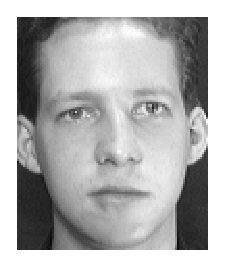
\includegraphics[scale=1.00]{img/original.eps}}
%   \caption{Immagini dopo 200 iterazioni a confronto}
% \end{figure}

\begin{figure}[h]
  \centering
  \subfigure[Senza pesi]
  {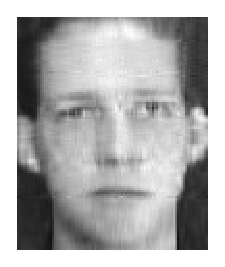
\includegraphics[trim = 5mm 20mm 5mm 12mm, clip=true, scale=1.70]{img/singUV_noW_200.eps}}
  \subfigure[Pesi centrati]
  {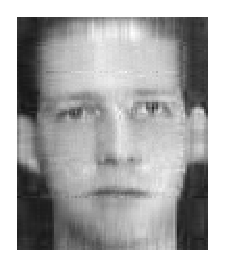
\includegraphics[trim = 5mm 20mm 5mm 12mm, clip=true, scale=1.70]{img/singUV_200.eps}}
  \subfigure[Originale]
  {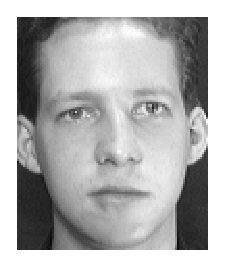
\includegraphics[trim = 5mm 20mm 5mm 12mm, clip=true, scale=1.70]{img/original.eps}}
  \caption{200 iterazioni, occhi a confronto}
\end{figure}

\begin{figure}[h]
  \centering
  Negativi a confronto:
  \subfigure
  {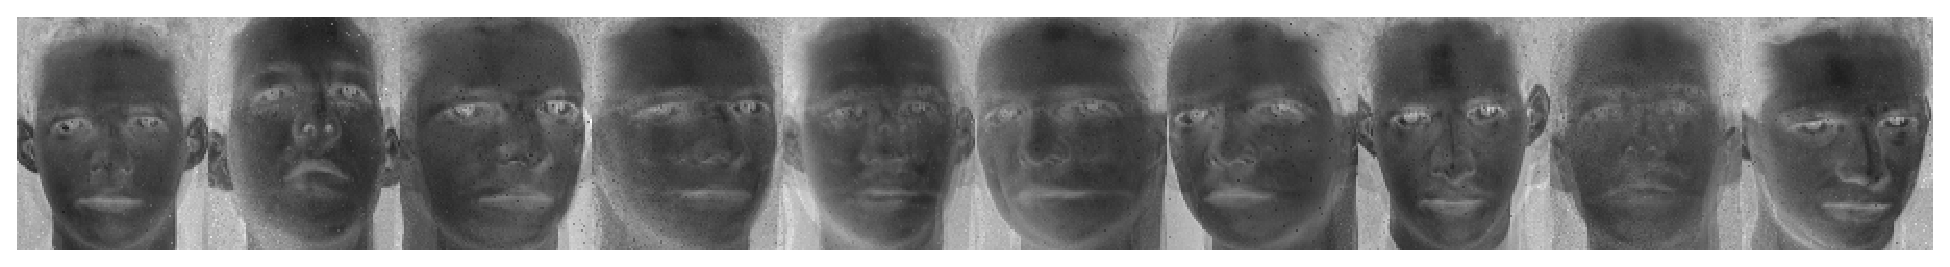
\includegraphics[scale=0.40]{img/negUV_noW.eps}}
  \subfigure
  {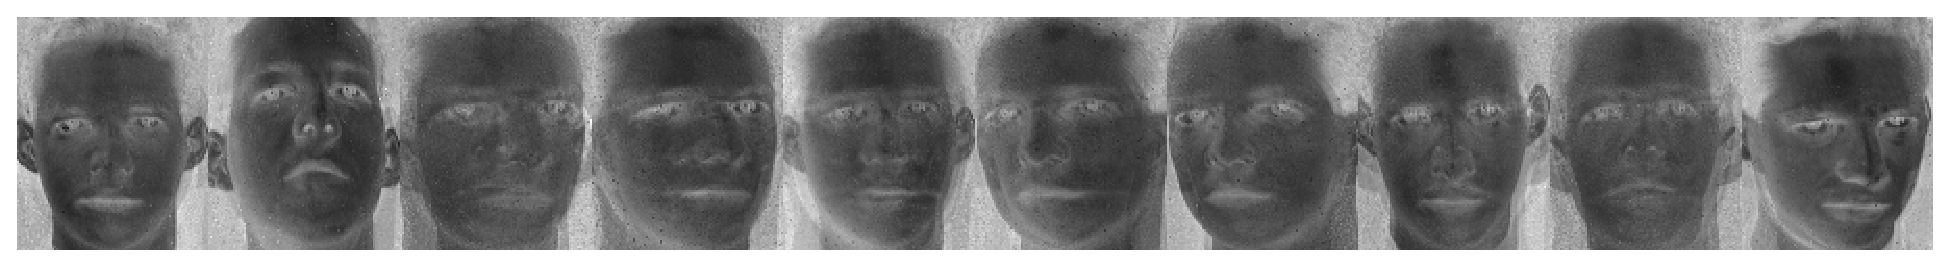
\includegraphics[scale=0.40]{img/negUV.eps}}
  % \vspace{2mm}
  \subfigure
  {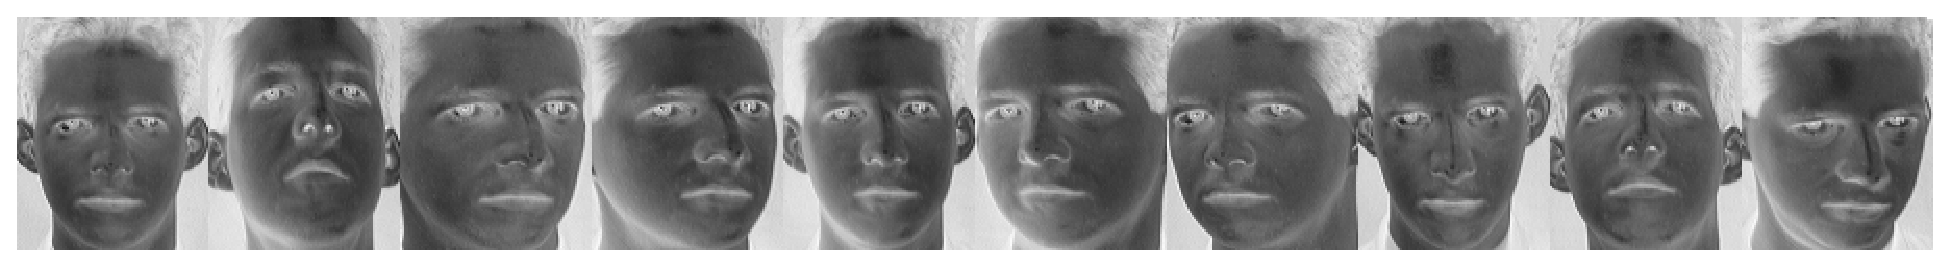
\includegraphics[scale=0.40]{img/negA.eps}}
  \caption{dall'alto: Negativi senza pesi, Negativi con pesi centrati, Originale}
\end{figure}

\clearpage{} % stampa pure quello che ti manca
%\nocite{*}
\begin{thebibliography}{}
 \bibitem{orlfacedb}{%
     Olivetti Research Laboratory,
     \emph{\texttt{ORL} face database},
     Cambridge University Computer Laboratory,
     between April 1992 and April 1994, \verb-http://www.cl.cam.ac.uk/research/dtg/attarchive/facedatabase.html-
   }\label{ORL}

 \bibitem{pgma2pgmb}{%
     John Burkardt,
     \emph{\texttt{PGMA TO PGMB}},
     under GNU LGPL Licence,
     March 2011, \verb-http://people.sc.fsu.edu/~jburkardt/cpp_src/pgma_to_pgmb/pgma_to_pgmb.html-
   }\label{itm:A2B}

 \bibitem{pgmaio}{%
     John Burkardt,
     \emph{\texttt{PGMA IO}},
     under GNU LGPL Licence,
     December 2005, \verb-http://people.sc.fsu.edu/~jburkardt/f_src/pgma_io/pgma_io.html-
   }\label{itm:IO}

 \bibitem{libnmf}{%
     A. Janecek, S. Schulze Grotthoff, W.N. Gansterer,
     \emph{\texttt{LIBNMF} – A LIBRARY FOR NONNEGATIVE MATRIX FACTORIZATION},
     University of Vienna, Austria,
     Faculty of Computer Science,
     Research Lab Computational Technologies \& Applications,
     from Computing and Informatics Volume 30, 2011
   }\label{libnmf}

\end{thebibliography}



\end{document}

